%=======================02-713 LaTeX template, following the 15-210 template==================
%
% You don't need to use LaTeX or this template, but you must turn your homework in as
% a typeset PDF somehow.
%
% How to use:
%    1. Update your information in section "A" below
%    2. Write your answers in section "B" below. Precede answers for all 
%       parts of a question with the command "\question{n}{desc}" where n is
%       the question number and "desc" is a short, one-line description of 
%       the problem. There is no need to restate the problem.
%    3. If a question has multiple parts, precede the answer to part x with the
%       command "\part{x}".
%    4. If a problem asks you to design an algorithm, use the commands
%       \algorithm, \correctness, \runtime to precede your discussion of the 
%       description of the algorithm, its correctness, and its running time, respectively.
%    5. You can include graphics by using the command \includegraphics{FILENAME}
%
\documentclass[11pt]{article}
\usepackage{amsmath,amssymb,amsthm}
\usepackage{tikz}
\usetikzlibrary{arrows,positioning, calc}
\tikzstyle{vertex}=[draw,fill=black!15,circle,minimum size=20pt,inner sep=0pt]
\usepackage{graphicx}
\usepackage[margin=1in]{geometry}
\usepackage{fancyhdr}
\usepackage{mathtools}
\usepackage{placeins}
\usepackage{listings}
\usepackage{color}
\usepackage{forest}
\usepackage{tikz}
\usepackage{caption}
\usepackage{mathtools}
\DeclarePairedDelimiter{\ceil}{\lceil}{\rceil}
\DeclarePairedDelimiter{\floor}{\lfloor}{\rfloor}

\definecolor{dkgreen}{rgb}{0,0.6,0}
\definecolor{gray}{rgb}{0.5,0.5,0.5}
\definecolor{mauve}{rgb}{0.58,0,0.82}

\lstset{frame=none,
  language=Java,
  aboveskip=3mm,
  belowskip=3mm,
  showstringspaces=false,
  columns=flexible,
  basicstyle={\small\ttfamily},
  numbers=none,
  numberstyle=\tiny\color{gray},
  keywordstyle=\color{blue},
  commentstyle=\color{dkgreen},
  stringstyle=\color{mauve},
  breaklines=true,
  breakatwhitespace=true,
  tabsize=3
}

\setlength{\parindent}{0pt}
\setlength{\parskip}{5pt plus 1pt}
\setlength{\headheight}{13.6pt}
\newcommand\question[2]{\vspace{.25in}\hrule\textbf{#1 #2}\vspace{.5em}\hrule\vspace{.10in}}
\renewcommand\part[1]{\vspace{.10in}\textbf{(#1)}}
\newcommand\algorithm{\vspace{.10in}\textbf{Algorithm: }}
\newcommand\correctness{\vspace{.10in}\textbf{Correctness: }}
\newcommand\runtime{\vspace{.10in}\textbf{Running time: }}
\pagestyle{fancyplain}
\lhead{\textbf{\NAME}}
\chead{\textbf{HW\HWNUM}}
\rhead{\today}
\begin{document}\raggedright
%Section A==============Change the values below to match your information==================
\newcommand\NAME{Sean Connor (443-414-5111)}  % your name
\newcommand\HWNUM{ PA2}              % the homework number
%Section B==============Put your answers to the questions below here=======================
\question{Analysis}{}
\part{a} 
The median-of-three partitioning method presented here is implemented using three functions - one to calculate the median of three numbers, one to swap the median with the last value in the array if necessary, and one to actually partition the array. These functions are presented below.
\begin{lstlisting}
/* Method to calculate median */
Median(int i, int j, int k){
	
	int temp;
	
	if (i > j){
		temp = i;
		i = j;
		j = temp;
	}
	if (i > j){
		temp = j;
		j = k;
		k = temp;
	}
	if (i > j){
		temp = i;
		i = j;
		j = temp;
	}
	
	return j;
	
}

/* Method to swap median with element at last index */
MO3-Swap(int[] A, int p, int r){
	
	x = Median(A[p], A[r], A[floor((p+r)/2)]);
	
	if (A[p] == x){
		exchange(A[p], A[r]);
	}
	
	if (A[floor((p+r)/2)] == x){
		exchange(A[floor((p+r)/2)], A[r]);
	}	
	
}

/* Method to partition array */
Partition(int[] A, int p, int r){
	
	MO3-Swap(A,p,r);
	x = A[r];
	i = p - 1;
	
	for (int j = p; j < r; j++){
		if (A[j] <= x){
			i++;
			exchange(A[i], A[j]);
		}
	}
	
	exchange (A[i+1], A[r]);
	
	return i + 1;
	
}
	
\end{lstlisting}

\part{b}
The worst-case performance remains the same - that is, O($n^2$). This is described well on page 175 of CLRS. The difference is that with median-of-three partitioning, the case where an array consists of all duplicate entries is the is the only case where the performance is minimized, and it seems to me that this would be a very rare case. 

Performance is still O($n^2$) if A[p], A[r], and A[$\floor{\frac{p+r}{2}}$] are \textit{always} the three lowest or three highest values in the array. In this case, the partition will produce one subproblem with one element and one subproblem with $n-2$ elements. The sum of the costs incurred at each level can be modeled as a summation of consecutive odd integers from 1 to N - this is given by $\ceil{\frac{n}{2}}^2$, and it is clear that this evaluates to O($n^2$).

The benefit of median-of-three partitioning is that it improves the likelihood of obtaining a good partitioning and reduces the probability of achieving worst-case performance. It \textit{does not} improve the best case performance of quicksort, and so the time complexity of quicksort with median-of-three partitioning is still $\Theta$(n lg n).

\part{c}
Using quicksort with median-of-three partitioning on a pre-sorted dataset results in the best case performance, which is $\Theta$(n lg n). The value found at A[$\floor{\frac{p+r}{2}}$] will always be the median, and will always provide the optimal partition of the array. The recurrence relation for this optimal split is given by the following:
\begin{equation}
T(n) = 2T\left(\frac{n}{2}\right) + \Theta(n).
\end{equation}
Figure 1 shows how sorted, reverse-sorted, and random ordering all follow n lg n when utilizing the median-of-three partitioning method.

\part{d} 
All code is provided. The performance of quicksort using both the median-of-three partitioning method and the partitioning method included in CLRS is evaluated. In addition, an additional important change was made. When testing the performance for high values of n (n >= 10000), the standard recursive quicksort method would produce StackOverflowError. To prevent this error, a partial recursive method with implemented that would recurse only on the smaller partition. This change allowed proper functioning of quicksort up to the highest value of n tested (n = 100000). All in all, performance testing was done on all combinations of quicksort (default vs median-of-three partitioning, full vs partial recursion) and ordered, reverse-ordered, random, all duplicate, and 10\% duplicate datasets with four different values of n for each (n=100, 1000, 10000, and 100000). 

A few notes. First, the random, sorted, and reverse-sorted datasets do not contain any duplicate values. In addition, the 10\% duplicate datasets are repeating - for example, for the n=100 dataset, the order is 1-2-3-4-5-6-7-8-9-10-1-2-3-4-5-6-7-8-9-10-... . Finally, the performance evaluation for the random dataset was averaged over five runs. In this, an important observation is that the coefficient of variation for performance of random datasets was less than 7\% for all n.

Performance was evaluated by tracking the number of calls of the exchange() method and by tracking the number of calls of the quicksort() method. Figures 1-4 provide an overview of the performance.

From this, it is clear that the median-of-three partitioning method provides a significant improvement for quicksort versus simply choosing the last element as the partition. However, it is also important to implement the partial recursion method over the full recursion method in order to avoid recursive stack overflow. There is a slight hit to performance; however, I believe this would be a worthwhile modification if it prevents error.

\begin{figure} [htbp!]
	\centering
	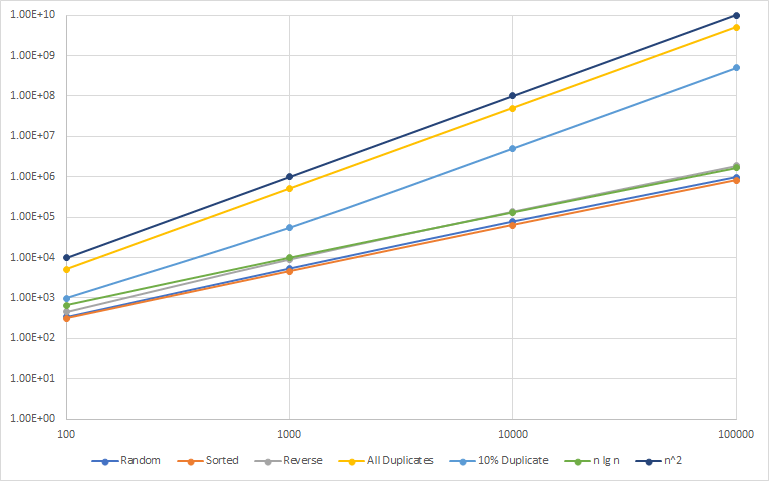
\includegraphics[width=\textwidth]{3Part}
	\caption{Performance of quicksort using the median-of-three partitioning method and partial recursion. }
\end{figure}

\begin{figure} [htbp!]
	\centering
	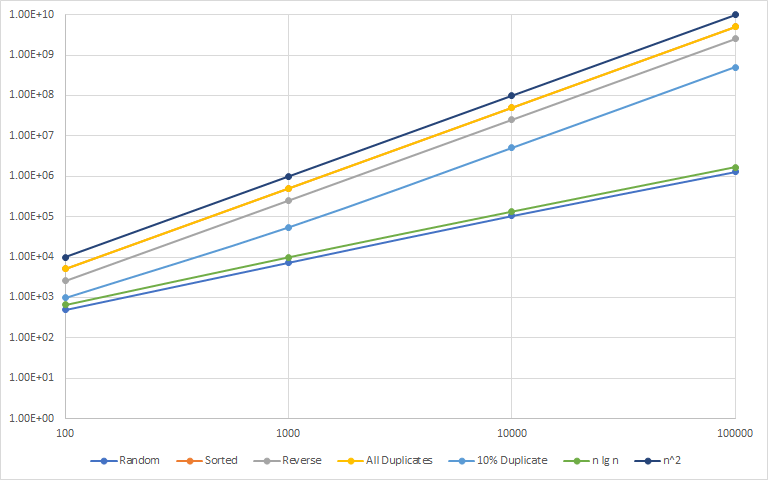
\includegraphics[width=\textwidth]{regPart}
	\caption{Performance of quicksort using the regular partitioning method and partial recursion. }
\end{figure}

\begin{figure} [htbp!]
	\centering
	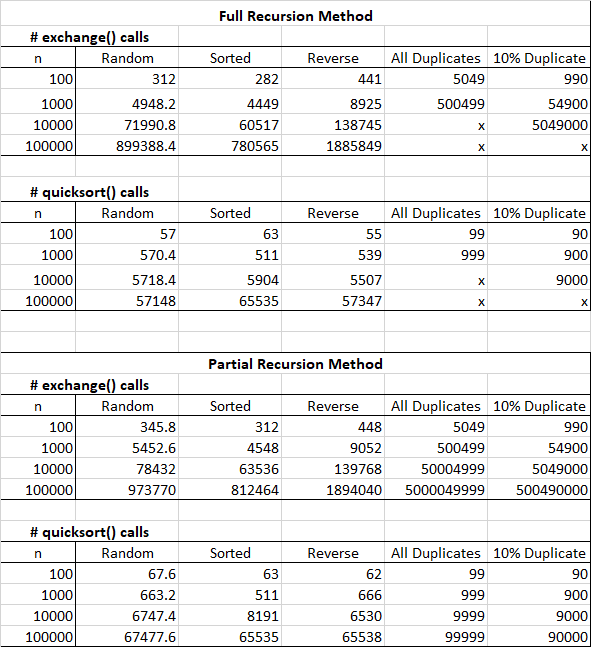
\includegraphics[width=6in]{3Part-table}
	\caption{Performance overview of quicksort using the median-of-three partitioning method.}
\end{figure}

\begin{figure} [htbp!]
	\centering
	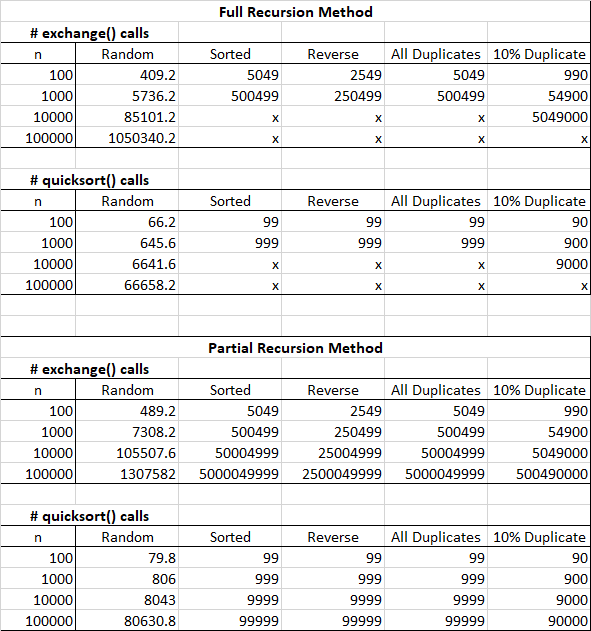
\includegraphics[width=\textwidth]{regPart-table}
	\caption{Performance of quicksort using the regular partitioning method.}
\end{figure}

\clearpage

\section{Appendix}
Here follows the ``full recursive'' quicksort method.
\begin{lstlisting}
if (p < r) {
	count++;
	long[] data = part.partition(array, p, r, ops);
	int q = Math.toIntExact(data[0]);
	ops = data[1];
	quicksort(array, p, q - 1);
	quicksort(array, q + 1, r);
}
\end{lstlisting}

Here follows the ``partial recursive'' quicksort method.
\begin{lstlisting}
while(p<r){
	count++;
	long[] data = part.partition(array, p, r, ops);
	int q = Math.toIntExact(data[0]);
	ops = data[1];
	
	if (q - p <= r - (q + 1)){
		quicksort(array, p, q);
		p = q + 1;
	}
	else{
		quicksort(array, q + 1, r);
		r = q - 1;
	}
}
\end{lstlisting}


\end{document}









